%%%%%%%%%%%%%%%%%%%%%%%%%%%%%%%%%%%%%%%%%%%%%%%%%%%%%%%%%
\section{Scenario}
\label{sec:scenario}

The tests take place in the \iterm{RoboCup@Home arena}. In addition, particular tests are situated outside the arena, e.g., in a previously unknown public place. The following rules are related to the \iterm{RoboCup@Home arena} and its contents. 

\subsection{RoboCup@Home arena}
The \iterm{RoboCup@Home arena} is a realistic home setting (apartment) consisting of inter-connected rooms like, for instance, a living room, a kitchen, a bath room, and a bed room. 
Depending on the Local Organization, there may be multiple apartments which may be different to each other.
Robot must be prepared to perform any task in any arena, not the same arena every time. 

The arena is decorated and dressed to resemble a home in which one could live, with as much of the necessities and decorations one might find in a normal home. 
Please do note that what is considered as \quotes{normal} may greatly vary by culture and on the location where the RoboCup event is hosted. 
For some examples on items one may find in the arena, see \refsec{chap:arena-decorations-appendix}

% \subsection{Team area}\label{rule:scenario_team_area}

% \todo{remove? does not depend on the rules, but on local organization }
% The maximum number of people to register per team is unlimited, but
% the organization only provides space for \emph{four} (4) persons to
% work at tables in the team area. 
% \todo{this is actually more an additional note for the registration information}

\subsection{Walls, doors and floor}
\label{rule:scenario_walls}

The indoor home setting will be surrounded by high and low \Term{walls}{Arena walls}. These walls will be built up using standard fair construction material.

\begin{enumerate}
	\item \textbf{Walls:} Walls have a minimum height of \SI{60}{\centi\meter}. A maximum height is not specified, but should be chosen so that the audience is able to watch the competition.\\
	Walls will be fixed and are likely to be not modified during the competition (see \refsec{rule:scenario_changes}). 

	\item \textbf{Doors:} There will be at least two entry/exit \Term{doors}{Arena doors} connecting the outside of the scenario. These doors are used as starting points for the robots (see \refsec{rule:start_position}).
	% At least one of the entrances will be a door with a handle (not a knob).\
	There will be also another door inside the scenario with a handle (not a knob) between any two rooms. Doors with handle (not a knob) may be closed at any time, it is expected robots be able to open them.

	\item \textbf{Floor:} The floor of the arena as well as the doorways of the arena are even. That is, there will be no significant steps or even stairways. However, minor unevenness such as carpets, transitions in floor covering between different areas, and minor gaps (especially at doorways) must be expected.

	\item \textbf{Appearance:} Floor and walls are mainly uni-colored but can contain texture, e.g., a carpet on the floor, or a poster or picture on the wall.\\
	Although being unlikely at the moment, transparent elements are also possible. 
\end{enumerate}


\subsection{Furniture}
\label{rule:scenario_furniture}

The arena will be equipped with typical objects (furniture) that are not specified in quantity and kind. The minimal configuration consists of 
\begin{itemize}
	\item a small dinner table with two chairs, 
	\item a couch, 
	\item an open cupboard or small table with a television and remote control, 
	\item a cupboard or shelf (with some books inside), and
	\item a refrigerator in the kitchen (with some cans and plastic bottles inside). 
\end{itemize}
A typical arena setup is shown in \reffig{fig:scenario_arena}.

\begin{figure}[tbp]
	\centering
	\subfloat[Typical arena]{\label{fig:scenario_arena}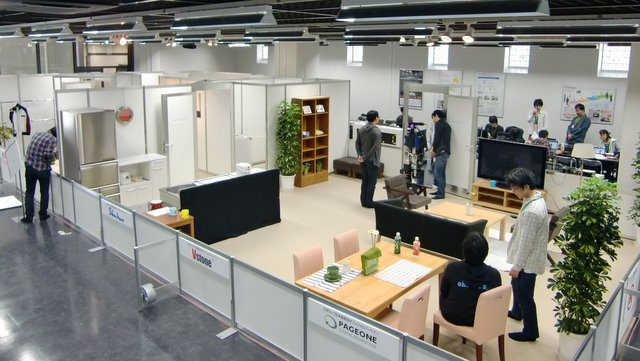
\includegraphics[height=46mm]{images/typical_arena.jpg}} ~ 
	\subfloat[Typical objects]{\label{fig:scenario_objects}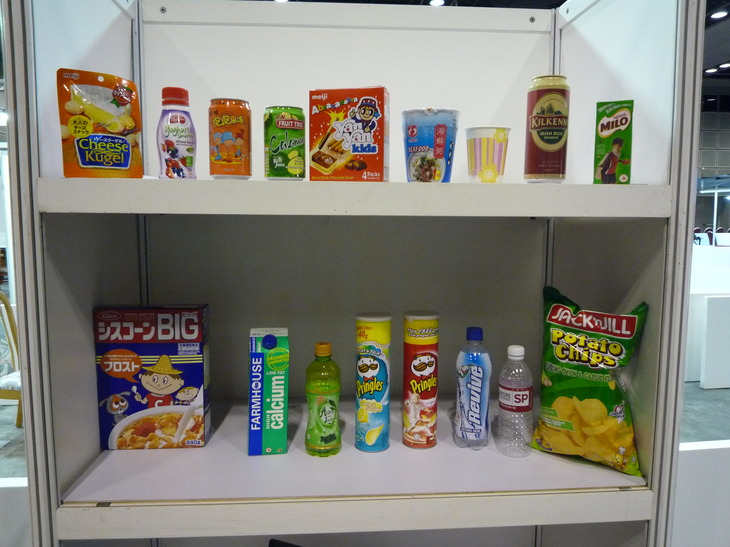
\includegraphics[height=46mm]{images/typical_objects.jpg}}
	\caption{Scenario examples: (a) a typical arena, and (b) typical objects.}
	\label{fig:arena}
\end{figure}



\subsection{Changes to the arena}
\label{rule:scenario_changes}

Since the robots should be able to function in the real world the scenario is not fixed and might change without further notice.
\begin{enumerate}
	\item \textbf{Major changes:} 
	The arena is meant to be a simulated apartment. 
	The furniture might be moved around between tests. 
	This includes furniture that is a named location (see \refsec{rule:scenario_names}).
	As in a normal home, furniture is not very likely to move from one room to another and is unlikely to be moved to the other side of a room.
	However, a couch or table may be rotated, moved to its side etc. 
	Walls will stay in place and rooms will not change function.
	Passages might be blocked and cleared. 
	One hour before a test slot begins no \iterm{major changes} will be made.
	This time will be shortened in the future. 
	\item \textbf{Minor changes:} In contrast to major changes, \iterm{minor changes} like, for instance, slightly moved chairs cannot be avoided and may happen at any time (even during a test). 
\end{enumerate}


%%%%%%%%%%%%%%%%%%%%%%%%%%%%%%%%%%%%%%%%%%%%%%%%%%%%%%%%%%%%%%%%%%
%
% Objects section.
%
% Revisited by Mauricio Matamoros for 2015
%
%%%%%%%%%%%%%%%%%%%%%%%%%%%%%%%%%%%%%%%%%%%%%%%%%%%%%%%%%%%%%%%%%%
\def\NumObjects{10\ }
\def\NumLocations{20\ }
\def\NumNames{20\ }

\subsection{Objects}
\label{rule:scenario_objects}
Some tests in the RoboCup@Home league involve object manipulation and recognition. These \iterm{objects} resemble items usually found in household environments like, for instance, soda cans, coffee mugs or books. An example of objects used in a previous competition can be seen in \reffig{fig:scenario_objects}.

Objects are divided in five main groups:

\begin{enumerate}
	\item \textbf{\iterm{Known objects}:} Objects with no noticeable difference among peers. \textit{Known objects} tend to be artificial and regular shaped, such as coke cans, beer bottles, cereal boxes, etc.~A set of copies of these objects is provided before the competition for training.

	\item \textbf{\iterm{Alike objects}:} Objects with slight differences among peers (e.g.~color, size, shape). \textit{Alike objects} tend to be natural and similar to each other, but not equal; for example: apples, bananas, rags, etc.~A specimen of these objects is provided before the competition for training.

	\item \textbf{\iterm{Containers}:} Objects which can contain, transport or be filled with other objects or their content, such as baskets, bowls, bags, trays, etc.~. As with \textit{known objects}, \textit{containers} are known beforehand with no noticeable difference among peers, and a copy is provided before the competition for training.

	\item \textbf{\iterm{Special objects}:} Objects require a proper identification and special handling (not necesarily grasping), operation or interaction for accomplishing a particular task. Examples of special objects are: door handles, chairs, walking sticks, poles, etc.~Notice that a copy of these objects may not be available beforehand for previous training.

	\item \textbf{\iterm{Unknown objects}:} Any other object that is not known beforehand but can be grasped or handled.
\end{enumerate}

The following general rules for objects apply:

\begin{enumerate}
	\item \textbf{Object category:} Each object will be assigned to an \iterm{object category}. The objects \quotes{apple} and \quotes{banana} may be of class \quotes{fruits} for example.

	\item \textbf{Object (category) locations:} An \iterm{object location} object will be assigned to each\iterm{object category}. For example, Objects categorized as \quotes{fruits} may be usually found on the \quotes{kitchen table}, and unknown objects \quotes{unknown} may be usually found on the \quotes{trash bin}.

	\item \textbf{Announcement:} The TC makes the set of \iterm{objects}, including their names, categories, and usual locations; available during the setup days. 
	
	\item \textbf{Placement:} \nterm{object placement} Unless stated otherwise, in manipulation tasks, the objects will be positioned at \iterm{manipulation locations} and less than \SI{15}{\centi\meter} away from the border of the surface they are located at. There will be at least \SI{5}{\centi\meter} space around each object.
\end{enumerate}

\paragraph*{Important note:} It is not allowed to modify any of the objects provided for training. Also, teams are not allowed to keep more than 5 the objects provided for training at a time nor retaining it for more than one hour.

\subsubsection{Containers}
The TC will provide at least three different types of containers to be used in the tests.

\begin{itemize}
	\item \textbf{Pouring containers:} Such as a bowls, glasses, or other objects in which liquids and grains can be poured.

	\item \textbf{Storage containers:} Such as bags or boxes in which objects can be stored or retrieved.\\
	Bags used during the competition are rigid and with clearly visible standing handles; more likely made of paper and in bright colors (See Figure \ref{fig:scenario_container_bag}).

	\item \textbf{Transport containers:} Such as trays in which objects can be neatly arranged for transport.
\end{itemize}

Although there are no restrictions on a container size, appearance or weight; however, it can be expected that the selected containers be lightweight, with handles, and easily manipulable by a human using either one or both hands.

\begin{figure}[H]
	\centering
	\subfloat[Bright-colored paper bags]{
		\label{fig:scenario_container_bag}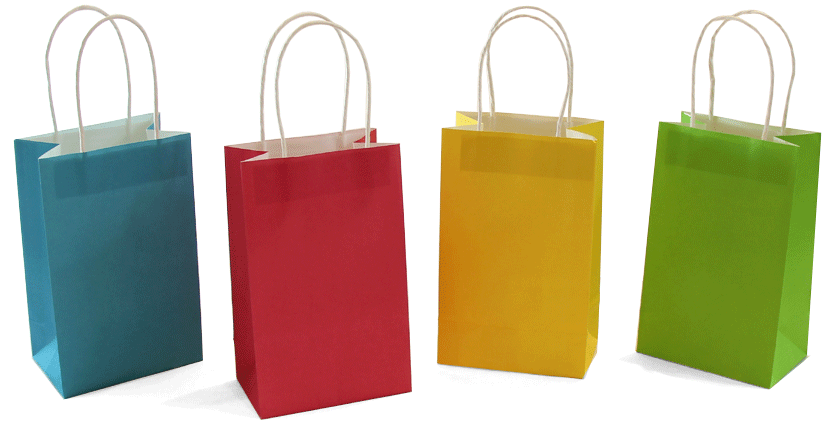
\includegraphics[width=0.33\textwidth]{images/container_paper_bag.png}}~
	\subfloat[Cereal bowls]{
		\label{fig:scenario_container_bowl}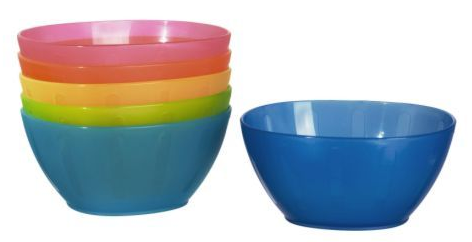
\includegraphics[width=0.33\textwidth]{images/container_bowl.png}}~
	\subfloat[Serving tray]{
		\label{fig:scenario_container_tray}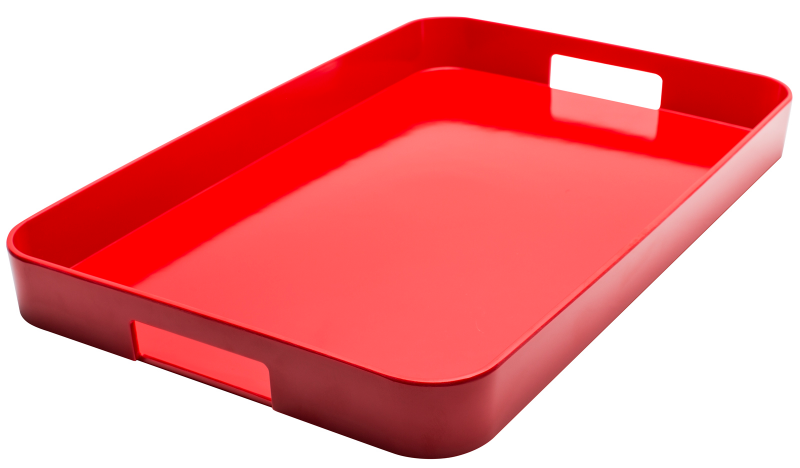
\includegraphics[width=0.33\textwidth]{images/container_tray.png}}
	\caption{Example of object containers}
	\label{fig:scenario_containers}
\end{figure}

\paragraph*{Custom containers.}
\label{rule:custom_containers}
It is allowed that a team provide a \iterm{custom container} adapted to be used by the robot, considering the following:
\begin{enumerate}
	\item Custom containers must be approved by the TC during during the \iterm{Robot Inspection} (see \refsec{sec:robot_inspection}).
	\item Custom containers must \emph{not} have any kind of artificial marks, sensors, or electronic devices.
	\item Penalties may apply for the use of custom containers. The TC may establish special penalties during the \iterm{Robot Inspection}. The default penalties applicable to any task involving a container are as follows.
	\begin{itemize}
		\item Special color on an otherwise unmodified two-hand manipulable container: 75\% of the points.
		\item Special color on an otherwise unmodified single-hand manipulable container: 50\% of the points.
		\item Specially designed or adapted two-hand manipulable container (e.g.~special handles): 50\% of the points.
		\item Specially designed or adapted single-hand manipulable container (e.g.~special handle): 25\% of the points.
		\item Two-hand manipulable container adapted to be used \textit{single-handed}: 25\% of the points.
		\item On-robot mounted container: 0 points.
	\end{itemize}
	\textbf{Notes:} Trays are considered two-hand manipulable containers, while most bowls and dishes are considered single-hand manipulable container unless they are too big. Color patterns are allowed as long as they look natural (e.g.~\textit{barber sign colored} handles are allowed, but black and white bar-code like handles are not). Penalties does not stack, the most meaningful modification is considered. 
\end{enumerate}

\subsubsection{Predefined objects}
The TC will compile a list of at least \NumObjects objects (including both \iterm{known objects} and \iterm{alike objects}) which will be available for training. There are no restrictions on an object size, appearance or weight; however, it can be expected that the selected objects are easily manipulable by a human using a single hand.

Note that, any object not previously announced by the TC is automatically considered an unknown object for scoring purposes (e.g.~ornamentation).

%%%%%%%%%%%%%%%%%%%%%%%%%%%%%%%%%%%%%%%%%%%%%%%%%%%%%%%%%%%%%%%%%%
%
% Predefined locations section.
%
%%%%%%%%%%%%%%%%%%%%%%%%%%%%%%%%%%%%%%%%%%%%%%%%%%%%%%%%%%%%%%%%%%

\subsection{Predefined locations}
\label{rule:scenario_locations}

Some tests in the RoboCup@Home league involve \iterm{predefined locations}. 
These may include places like a \quotes{bookshelf} or a \quotes{dining table}, as well as certain objects such as a \quotes{television}, or the \quotes{front door}. 

\begin{enumerate}
	\item \textbf{Definition:} The TC will compile a list of predefined locations. There are no restrictions on which parts of the arena will be selected as a predefined location.

	\item \textbf{Location classes:} Each location will be assigned to a \iterm{location class}. The objects \quotes{couch} and \quotes{arm chair} may be of class \quotes{seat} for example. 

	\item \textbf{Announcement:} The TC makes the set of locations (and their names and classes) available during the setup days.

	\item \textbf{Position:} The positions of locations are \emph{not} necessarily fixed (see \refsec{rule:scenario_changes}).

	\item \textbf{Manipulation locations:} The TC will mark at least \NumLocations locations out of the set of predefined locations as being \iterm{manipulation locations}. Whenever a test involves manipulation, the object to manipulate will be placed at one of the manipulation locations. 
\end{enumerate}



\subsection{Predefined rooms}
\label{rule:scenario_rooms}
Some tests in the RoboCup@Home league involve \iterm{predefined rooms}. 
\begin{enumerate}
	\item \textbf{Definition:} The TC will compile a list of room names.
	\item \textbf{Announcement:} The TC makes the set of rooms available during the setup days.
\end{enumerate}



\subsection{Predefined (person) names}\label{rule:scenario_names}

Some tests in the RoboCup@Home league involve \iterm{predefined names} of people. 

\begin{enumerate}
	\item \textbf{Definition:} The TC will compile a list of \NumNames predefined names. The names are \SI{50}{\percent} male and \SI{50}{\percent} female, and taken from the (current) most common first names in the United States.\\
	In order to ease speech recognition, it is tried to select names to be phonetically different from each other.

	\item \textbf{Announcement:} The TC makes the set of names available during the setup days.
	\item \textbf{Assignment:} When a test involves interacting with persons (using a person's name), all involved persons are assigned names by the referees before the test. 
\end{enumerate}

Typical names are, for example, James, John, Robert, Michael and William as male names; Mary, Patricia, Linda, Barbara and Elizabeth as female names.

% MAURICIO @2017
% Separated file for better control
%% %%%%%%%%%%%%%%%%%%%%%%%%
\subsection{Wireless network}
\label{rule:scenario_wifi}

For wireless communication, an \iterm{arena network} is provided. The actual infrastructure depends on the local organization. 

\begin{itemize}
	\item To avoid interference with other leagues, this \iterm{arena network} has to be used for communication only. It is not allowed to use the above or any other WiFi network for personal use at the venue.
	\item During the competitions, only the active team is allowed to use the \iterm{arena network}. 
	\item The organizers cannot guarantee reliability and performance of wireless communication. Therefore, teams are required to be ready to setup, start their robots and run the tests even if, for any reason, network is not working properly.
\end{itemize}

Preferred situation:
\begin{itemize}
	\item The \iterm{arena network} consists of of several Virtual Local Area Networks (VLANs), one for each team. 
	\item The traffic from the robot inside the arena is separated into the corresponding team's VLAN as soon as possible, e.g. at the wireless acces point.This may require that each team has it's own SSID, each of which gets routed into the corresponding VLAN. Each team has a network cable routed to their team area, which is also connected to the teams VLAN. On this cable, the team can set up their own router/switch/hub etc. which will be inside the team's VLAN. This way, one team's traffic and devices are completely separated from any other team, while any team can set up their own DHCP server etc. if they desire. 
	\item An Internet connection is preferably also available for every team. 
\end{itemize}
Each team has to bring its own LAN hub/switch and cables for routing inside the team area. 

In case the \iterm{arena network} is not functioning at the end of the first setup day, teams are allowed to set up their own networking equipment and wireless networks.

\paragraph*{Important note:} Different countries have different regulations for wireless equipment and the \iterm{arena network} has to obey these. 
It is up to the teams to have networking equipment that also adheres to these regulations. For example, if due to local regulations various WiFi channels are prohibited, it is a team's responsibility to be able to use different, allowed channels.

\paragraph*{Important note:} Any unapproved wireless device may be removed by the TC at any time.

% Local Variables:
% TeX-master: "../Rulebook"
% End:

% MAURICIO @2017
% We are not really using SmartHome devices anymore.
%\subsection{Smart Home Devices}
\label{rule:smarthomedevices}

The Organizing and Technical Committees in coordination with the Local Organization will compile a list of \iterm{Smart~Home} official devices that will be available in the arena and can be used in some tests for additional score.

At any time, only the Smart~Home devices provided by the Local Organization and approved by the Technical Committee may be used during competition.

\subsubsection{Smart~Home devices list announcement}
The list if Smart~Home devices will be provided to teams as soon as it becomes available and has been granted by the Local Organization and approved by the Technical Committee. 

This list must be announced at least one month prior the competition. In case that this list does not become available for that date, Smart~Home devices may still be present at the arena for testing, but no additional score can be achieved for its use. This is to maintain fair conditions among all teams.

\subsubsection{Technical specifications}
The list of \iterm{Smart~Home} official devices will include as much technical information as possible. However, before it becomes available you may assume the following considerations:

\begin{enumerate}
	\item \textbf{Interface:} Most Smart~Home devices interface wireless, often via R/F transmitters. When possible, the OC will provide an official interface via the \iterm{arena network}.
	\item \textbf{Operating voltage:} The operating voltage used will be the standard for the place of the competition (e.g.120V/60Hz for North America and 220V/50Hz for Europe). Please note that devices designed for other voltages/frecuencies may burn when plugged to the outlet.
	\item \textbf{Type of devices:} Mostly Smart~Home switches will be used (set on/off, read can not be guaranteed). For high bandwidth devices such as microphones or video cameras, an official interface (such as a ROS topic or web service) will be provided via the \iterm{arena network}.
\end{enumerate}

\subsubsection{Availability \& Scoring}
All test has been designed to optionally allow the use of Smart~Home devices and even grant bonus scoring for using this option. However, robots must be able to continue operating normally when there are no Smart~Home devices available. Therefore, it is unacceptable that a robot gets stuck or in some sort of deadlock while trying to operate those devices.

As stated in \refsec{rule:scenario_wifi}, organizers cannot guarantee reliability and performance of wireless communication. Therefore, in case of malfunction or communication problems with the Smart~Home devices, or any other issue which may affect scoring, no claims will be accepted by the EC/TC/OC, nor test will be repeated. The decision on if a team given points for using \iterm{Smart~Home} devices, is conducted by the \iaterm{Technical Committee}{TC}, and it reserves the rights of discarding Smart~Home related scoring.


% Local Variables:
% TeX-master: "../Rulebook"
% End:


% Local Variables:
% TeX-master: "../Rulebook"
% End:
